\documentclass[man]{apa6}
\usepackage{lmodern}
\usepackage{amssymb,amsmath}
\usepackage{ifxetex,ifluatex}
\usepackage{fixltx2e} % provides \textsubscript
\ifnum 0\ifxetex 1\fi\ifluatex 1\fi=0 % if pdftex
  \usepackage[T1]{fontenc}
  \usepackage[utf8]{inputenc}
\else % if luatex or xelatex
  \ifxetex
    \usepackage{mathspec}
  \else
    \usepackage{fontspec}
  \fi
  \defaultfontfeatures{Ligatures=TeX,Scale=MatchLowercase}
\fi
% use upquote if available, for straight quotes in verbatim environments
\IfFileExists{upquote.sty}{\usepackage{upquote}}{}
% use microtype if available
\IfFileExists{microtype.sty}{%
\usepackage{microtype}
\UseMicrotypeSet[protrusion]{basicmath} % disable protrusion for tt fonts
}{}
\usepackage{hyperref}
\hypersetup{unicode=true,
            pdftitle={Objectification in Action: Self- and Other-Objectification in Same-gender Interactions},
            pdfauthor={Randi L. Garcia, Kat Kyuchukova, Asha Hinson, \& Laneé Jung},
            pdfkeywords={Interpersonal sexual objectification, self-objectifiation, authenticity,
actual interactions, psychology of women, dyadic data analysis},
            pdfborder={0 0 0},
            breaklinks=true}
\urlstyle{same}  % don't use monospace font for urls
\usepackage{graphicx,grffile}
\makeatletter
\def\maxwidth{\ifdim\Gin@nat@width>\linewidth\linewidth\else\Gin@nat@width\fi}
\def\maxheight{\ifdim\Gin@nat@height>\textheight\textheight\else\Gin@nat@height\fi}
\makeatother
% Scale images if necessary, so that they will not overflow the page
% margins by default, and it is still possible to overwrite the defaults
% using explicit options in \includegraphics[width, height, ...]{}
\setkeys{Gin}{width=\maxwidth,height=\maxheight,keepaspectratio}
\IfFileExists{parskip.sty}{%
\usepackage{parskip}
}{% else
\setlength{\parindent}{0pt}
\setlength{\parskip}{6pt plus 2pt minus 1pt}
}
\setlength{\emergencystretch}{3em}  % prevent overfull lines
\providecommand{\tightlist}{%
  \setlength{\itemsep}{0pt}\setlength{\parskip}{0pt}}
\setcounter{secnumdepth}{0}
% Redefines (sub)paragraphs to behave more like sections
\ifx\paragraph\undefined\else
\let\oldparagraph\paragraph
\renewcommand{\paragraph}[1]{\oldparagraph{#1}\mbox{}}
\fi
\ifx\subparagraph\undefined\else
\let\oldsubparagraph\subparagraph
\renewcommand{\subparagraph}[1]{\oldsubparagraph{#1}\mbox{}}
\fi

%%% Use protect on footnotes to avoid problems with footnotes in titles
\let\rmarkdownfootnote\footnote%
\def\footnote{\protect\rmarkdownfootnote}


  \title{Objectification in Action: Self- and Other-Objectification in
Same-gender Interactions}
    \author{Randi L. Garcia\textsuperscript{1, 2}, Kat
Kyuchukova\textsuperscript{1, 2}, Asha Hinson\textsuperscript{1}, \&
Laneé Jung\textsuperscript{2}}
    \date{}
  
\shorttitle{Objectification in Action}
\affiliation{
\vspace{0.5cm}
\textsuperscript{1} Department of Psychology, Smith College\\\textsuperscript{2} Program in Statistical and Data Sciences, Smith College}
\keywords{Interpersonal sexual objectification, self-objectifiation, authenticity, actual interactions, psychology of women, dyadic data analysis}
\usepackage{csquotes}
\usepackage{upgreek}
\captionsetup{font=singlespacing,justification=justified}

\usepackage{longtable}
\usepackage{lscape}
\usepackage{multirow}
\usepackage{tabularx}
\usepackage[flushleft]{threeparttable}
\usepackage{threeparttablex}

\newenvironment{lltable}{\begin{landscape}\begin{center}\begin{ThreePartTable}}{\end{ThreePartTable}\end{center}\end{landscape}}

\makeatletter
\newcommand\LastLTentrywidth{1em}
\newlength\longtablewidth
\setlength{\longtablewidth}{1in}
\newcommand{\getlongtablewidth}{\begingroup \ifcsname LT@\roman{LT@tables}\endcsname \global\longtablewidth=0pt \renewcommand{\LT@entry}[2]{\global\advance\longtablewidth by ##2\relax\gdef\LastLTentrywidth{##2}}\@nameuse{LT@\roman{LT@tables}} \fi \endgroup}


\DeclareDelayedFloatFlavor{ThreePartTable}{table}
\DeclareDelayedFloatFlavor{lltable}{table}
\DeclareDelayedFloatFlavor*{longtable}{table}
\makeatletter
\renewcommand{\efloat@iwrite}[1]{\immediate\expandafter\protected@write\csname efloat@post#1\endcsname{}}
\makeatother

\authornote{Randi L. Garcia is in the Psychology Department
and the Statitsical and Data Sciences program at Smith College.

The data that support the findings of this study are available on
request from the corresponding author. The data are not publicly
available due to privacy or ethical restrictions.

Correspondence concerning this article should be addressed to Randi L.
Garcia, 415 Bass Hall, Smith College, Northampton, MA 01060. E-mail:
\href{mailto:rgarcia@smith.edu}{\nolinkurl{rgarcia@smith.edu}}}

\abstract{
Existing research on interpersonal objectification has focused mostly on
links between objectification, self-objectification, and negative
outcomes for women within mixed-gender interactions (Garcia, Earnshaw,
\& Quinn, 2016; Gervais, Sáez, Riemer, \& Klein, 2020). The purpose of
the present study was to extend past research on interpersonal
objectification to interactions between women. Women were brought into
the laboratory and interacted face-to-face in same-sex dyads. Dyadic
analysis (Kenny, Kashy, \& Cook, 2006) was utilized to detect whether
partners' objectification of each other affected state
self-objectification, as well as the resulting feelings of comfort and
authenticity during the interaction. Results revealed a significant
positive relationship between being objectified by a woman interaction
partner and women's own self-objectification (a partner effect). There
was no significant relationship between self-objectification and
interaction inauthenticity, but there were significant negative effects
of inauthenticity on career aspirations and relationship agency (actor
effects). The significant partner effect of objectification on
self-objectification suggests that women being objectified by other
women may result in feelings of self-objectification, and this finding
opens up questions for future research about how interpersonal
objectification might function in situations without an immediate male
gaze.


}

\begin{document}
\maketitle

Fredrickson and Roberts (1997)'s Objectification Theory, suggests that,
in addition to being steeped in a culture that objectifies women, women
are objectified in actual interpersonal encounters. The negative effects
of this interpersonal objectification for women have been theorized to
be the strongest under the \enquote{male gaze,} that is, when it is a
perceived or actual man doing the objectifying (Calogero, 2004; Gay \&
Castano, 2010; Gervais, Vescio, \& Allen, 2011), but what are the
consequences when a woman objectifies another woman in an interaction?
Psychological researchers studying the sexual objectification of women
have in recent years explored the interpersonal process of the
objectification, finding evidence for \emph{self}-objectification in the
target as a proximal consequence of being objectified (Garcia et al.,
2016; Riemer, Sáez, Brock, \& Gervais, 2020; Strelan \& Pagoudis, 2018).
In a recent review, Gervais et al. (2020) organized the extant
literature on interpersonal self-objectification and proposed a
theoretical model called the Social Interaction Model of Objectification
(SIMO). The SIMO focuses on understanding mixed-gender interactions,
acknowledging the patriarchal power structure embedded in these mixed
interactions, but can it be extended to interactions among women?
Although there is evidence that women can objectify other women
(Gervais, Holland, \& Dodd, 2013; Loughnan et al., 2015; Puvia \& Vaes,
2013), studies investigating the process of interpersonal
objectification in interactions between women is scarce.

The current study uses a face-to-face interaction methodology to being
to answer a series of research questions about interpersonal
objectification among women: Is objectification by a female interaction
partner related to an increase in self-objectification for the woman
being objectified? Does objectification by a woman have the same
downstream negative consequences for women as being objectified by a
male interaction partner? The current study addresses these questions by
investigating interpersonal objectification among interacting pairs
where both partners identify as women.

\subsection{Self-Objectification}\label{self-objectification}

Self-objectification is a psychological process that translates the
experiences of interpersonal objectification (Gervais et al., 2020;
Loughnan, Baldissarri, Spaccatini, \& Elder, 2017) into negative mental
health outcomes (e.g., interaction inauthenticity, anxiety, lower
self-esteem, and poor cognitive performance; Calogero, Tantleff-Dunn, \&
Thompson, 2011; Moradi \& Huang, 2008). Calogero et al. (2011) proposes
that self-objectification can be conceptualized as a learned trait, or
\emph{trait} self-objectification (TSO), whereby one adopts a habitual
third-person perspective on one's own appearance. Furthermore,
self-objectification can also be elicited momentarily, for example, when
viewing sexualized images in movies and magazines (Morry \& Staska,
2001), when trying on sexualizing clothing (B. L. Fredrickson, Roberts,
Noll, Quinn, \& Twenge, 1998), or during video chat when you believe
your interaction partner can only see your body (not face; Saguy, Quinn,
F Dovidio, \& Pratto, 2010). This momentary self-objectification is
referred to as \emph{state} self-objectification (SSO; Calogero et al.,
2011; Moradi \& Huang, 2008) and is characterized by feeling like a body
rather than a full self within a particular moment, instance, or
context.

Perhaps the most adverse negative consequence of interpersonal
objectification is that being objectified socializes girls and women to
routinely treat themselves as objects to be looked at and evaluated
(Bartky, 1990). There is experimental and observational evidence that
being objectified by another person during an interaction elicits SSO.
For example, Loughnan et al. (2017) found that for women, imagining a
time when they were objectified by another person caused reductions in
human traits attributed to the self, and notably, the gender of the
person doing the objectification was not a moderating factor. In
addition, in a mixed-gender dyadic study of actual interactions, Garcia
et al. (2016) found that men's reported objectification of their female
interaction partner was associated with increased self-objectification
in the female partner. Further, this negative effect of the men's
objectification on women's SSO was strongest for women higher in TSO.
The current study uses this same dyadic paradigm to study same-gender,
woman-woman interacting pairs.

\subsection{Women Objectifying Women}\label{women-objectifying-women}

Past research investigating women objectifying other women has focused
on the psychological conditions that lead women to objectify other
women. Harsey and Zurbriggen (2020) found that (trait)
self-objectification was related to the objectification of women to a
similar degree for male and female participants. Along the same lines,
Strelan and Hargreaves (2005) found that the more women self-objectify,
the more they objectify other women. Could the process work in the other
direction as well, that is, could objectification by a woman produce
(state) self-objectification, in a similar manner to objectification by
a man? Hill and Fischer (2008) assessed women's experiences of
objectification from men independently from women's experiences of
objectification from other women. They found that women may be
socialized not only to see themselves as objects, but perhaps to see
other women as objects as well. This process, however, was not confirmed
to occur during an actual interpersonal interaction. Thus, there is
evidence that women do objectify other women, indeed, Loughnan et al.
(2017) found that women objectify other women to a greater extent than
they objectify men. Women have also been found to objectify
(dehumanized) sexualized targets presented as images (Puvia \& Vaes,
2013), but very little is known about interpersonal sexual
objectification among women and what the effects of this objectification
might be. Past studies have found that objectification has more adverse
consequences for women than men (Gervais et al., 2011; Moradi \& Huang,
2008; Saguy et al., 2010), however, we do not know much about the effect
of the gender of the \emph{objectifyer} on these potential detrimental
outcomes.

\subsection{Interpersonal
Objectification}\label{interpersonal-objectification}

Studies have shown that within social encounters women are gazed at more
than men (Henley, 1977), often times feel \enquote{looked at} within
interpersonal interactions (Argyle \& Williams, 1969), and are likely to
internalize the objectifying gaze on their physical self (Puvia \& Vaes,
2013). As mentioned above, interpersonal objectification has been found
to have negative consequences for women. Gervais et al. (2011) found
that an objectifying gaze by a male interaction partner (confederate)
was associated with lower math performance for women than being
objectified by a female interaction partner. Gervais et al. (2020)
recently reviewed the research on interpersonal objectification and
organized our current theoretical understanding of this process in the
SIMO. What is clear from Gervais et al. (2020)'s review is that we know
little about women-on-women interpersonal objectification.

Past research has found that the experience of state
self-objectification in mixed-gender contexts (stranger and romantic;
Strelan and Pagoudis (2018); Meltzer (2020); Zurbriggen, Ramsey, and
Jaworski (2011)) has negative consequences for women, but what about in
the context of interactions with other women? Is the
self-objectification experienced in mixed-gender interactions associated
with the same negative process as that experienced in same-gender
interactions? The ample research demonstrating that the male gaze has a
particularly detrimental effect for women would suggest no (Calogero,
2004; Gay \& Castano, 2010; Gervais et al., 2011; Saguy et al., 2010),
but, there is evidence that women do objectify other women (Harsey \&
Zurbriggen, 2020; Loughnan et al., 2015; Puvia \& Vaes, 2013) and recent
experimental evidence suggests that the female gaze causes no less
self-objectification than the male gaze (Yilmaz \& Bozo, 2019). It would
be helpful to understand the consequences of this \emph{intra}group
objectification for women. When women objectify other women, does it
lead to self-objectification in the same way men's objectification of
women does (Garcia et al., 2016)? If so, does the self-objectification
experienced in these same-gender interactions have the same negative
consequences for authenticity in that interaction?

There is some evidence that reduced authenticity is a consequence of
self-objectification (Garcia et al., 2016; Terán, Jiao, \& Aubrey,
2020). A recent study has investigated the effect of
self-objectification on the reduction of relationship building skills in
general (including same-sex friendships) (Terán et al., 2020).
Authenticity reduction and interaction quality disruptions have also
been found in research on stigmatized-stigmatizer interactions (M. R.
Hebl \& Dovidio, 2005; Pearson et al., 2008; Richeson \& Shelton, 2003;
Shelton, Richeson, \& Salvatore, 2005), and we might view the experience
of being objectified in an interaction as a potential identity threat
situation (Gervais et al., 2020; Nadal \& Haynes, 2012). Further,
empirical evidence reveals that healthy relationship functioning
manifests through authenticity in romantic relationships (Brunell et
al., 2010), an intergroup context at least in heterosexual
relationships. Evidence for other adverse consequences of interpersonal
objectification include reductions in career aspirations (Garcia et al.,
2016) and a decrease in concentration and impairment in female cognitive
performance (Kahalon, Shnabel, \& Becker, 2018; D. M. Quinn, Chaudoir,
\& Kallen, 2011). These are also negative consequences found for women
under stereotype threat (Davies, Spencer, \& Steele, 2005). When a woman
is objectified by a man, and subsequently experiences
self-objectification, the intergroup nature and power differential of
this encounter might trigger threat. Thus, perhaps there are fewer
negative consequences when a woman is objectified by another woman. That
is, the intergroup threat literature might predict that woman-woman
interpersonal objectification processes diverge from mixed-gender
interpersonal objectification processes precisely because they are not
intergroup interactions (at least with respect to gender identity).

In summary, a woman objectified by another woman may not be having the
same negative consequences that cascade from situations that trigger
group-based identity threat (Deaux \& Major, 1987; Dovidio, Hebl,
Richeson, \& Shelton, 2006; M. R. Hebl \& Dovidio, 2005); however,
feeling like a body rather than a full human (higher SSO) in any
interaction, whether intergroup or intragroup, may be enough to reduce
women's feelings of authenticity and social competence, regardless of
the gender of the objectifyer (Terán et al., 2020; Tolman, Impett,
Tracy, \& Michael, 2006).

\subsection{The Current Study}\label{the-current-study}

In the current study, we sought to examine what occurs during an
interaction in which one or both partners are objectifying each other,
similarly to Garcia et al. (2016), but between same-gender interpersonal
interactions among women. Moreover, the current study uses a
face-to-face interaction paradigm and dyadic data analysis techniques to
examine the relationships for both women simultaneously. Although the
literature on intragroup objectification among women is small, the
results are mixed, and they do not cover interpersonal encounters, we
expected to replicate some of the results found in Garcia et al. (2016).
Most importantly, we predicted that being objectified by one's
interaction partner would be related to state self-objectification
(SSO). We also expected that TSO would moderate this relationship,
amplifying the positive association between being objectified and SSO
for women higher in TSO. Here we would like to note that Puvia and Vaes
(2013) would alternatively predict that women's tendency to
self-objectify (TSO) leads them to objectify other women (more
precisely, to dehumanize a sexualized woman). In addition, Strelan and
Hargreaves (2005) and Harsey and Zurbriggen (2020) would also predict
the TSO to other-objectification link, further theorizing that this
relationship is mediated by the woman's own state self-objectification
(SSO). Thus, the limited but extant literature on woman-woman
objectification points to a possible alternative model from the model
tested in the current study. Where appropriate, we report results
considering the causal directions implied by this alternative mediation
model.

We also tested whether SSO would, in turn, lead to feelings of
inauthenticity. The investigation of the SSO to inauthenticity
connection is considered exploratory given the lack of support for this
connection from the literature on identity threat in \emph{intra}group
interactions but support for this connection in the objectification
literature (Garcia et al., 2016; Rollero, 2016; Terán et al., 2020).
Regardless of whether there was an association between SSO and
inauthenticity, we hypothesized that feelings of inauthencity would be
associated with reduced feelings of agency in romantic relationships,
reduced career aspirations, and reduced cognitive performance. In
summary, we expected to find a positive relationship between
other-objectification by one's partner and state self-objectification.
We also expected to find a negative relationship between state-self
objectification and interaction authenticity, and that interaction
authenticity will be positively related to cognitive performance,
relationship agency, and career aspirations.

\section{Methods}\label{methods}

\subsection{Procedure}\label{procedure}

Except for the instructions given to participants, the procedure used
was identical to that in Garcia et al. (2016). In brief, that
methodology is that each participant arrived at the laboratory and were
then led into separate cubicles to prevent any communication between the
participants before the interaction. In addition, each participant was
screened for prior acquaintance to confirm that they had not met prior
to the study. They were asked to sign the consent form to participate,
and the study was described as follows: \enquote{This is a study looking
at how students form different types of relationships at college.} A
prompt on the computer screen told the participants that they were
assigned to the \enquote{College Relationships} condition and gave the
following instructions:

\begin{quote}
There are many types of relationships people form in college. During the
interaction, please think about your partner's potential as a romantic
partner. \textbf{Even if they are not the gender you are attracted to},
you can still judge their potential as a romantic partner. After the
interaction you will be asked to evaluate how dateable your partner is.
In other words, we would like to know if you think someone would date
your interaction partner. Also, your interaction partner will be
evaluating you in the same manner.
\end{quote}

\emph{All} participants were told that they were assigned to the
\enquote{College Relationships} condition. Self-objectification has been
found to occur after a mere relationship prime among women (Sanchez \&
Broccoli, 2008) because, in Western culture and beyond, women need to
look attractive to obtain and maintain successful relationships, thus,
the \enquote{College Relationships} condition may heighten
self-objectification and the evaluation of other women in a sexualized
way. The decision was made to ask even heterosexual women to judge their
fellow-woman partners for their potential as romantic partners. We felt
that this prompt would keep the study closest to a replication of the
previous Garcia et al. (2016) version of the study, and strengthen the
potential for objectification that would normally be low in the context
of a psychology laboratory. Recall that, past research has found that
heterosexual women are indeed able to evaluate other women's potential
as romantic partners (i.e., their sexual attractiveness; Puvia \& Vaes,
2013)---women may be unfortunately quite used to thinking about their
own \enquote{datability,} and we suspect this this habitual thought
pattern will translate to their thoughts about other women. Analyses
comparing levels of other-objectification between heterosexual and
non-heterosexual women are provided in the measures section below.

After receiving the \enquote{College Relationships} prompt, the two
participants were then brought into a larger interaction room where they
sat on stools prearranged to be approximately 1 meter apart. The
experimenter instructed the participants to \enquote{get to know each
other} for 10 minutes and then left the room. After 10 minutes, the
experimenter came back into the room and stopped the interaction. The
participants then went back to their individual cubicles and completed a
set of post-interaction measures. Participants were then thanked for
their participation and debriefed. More detail on this methodology can
be found in Garcia et al. (2016).

\subsection{Participants}\label{participants}

Thirty-two previously unacquainted dyads of self-identifying women
participated in this study. Data from two demographically similar higher
education institutions in the Northeast United States were combined to
create the final analysis sample (\emph{N =} 64) used in this study. In
the measures section that follows we refer to them as Sample 1 and
Sample 2. Sample 1 (\emph{N =} 24, or 12 pairs) is from a co-ed liberal
arts college and Sample 2 (\emph{N =} 40, or 20 pairs) is from a women's
liberal arts college. Initially, data was collected from both
same-gender and mixed-gender dyads at both institutions. Sample 1
originally consisted of 22 pairs, 12 men and 32 women. In Sample 2 there
were 23 pairs made up of 43 women and one man, as well as two
participants who did not identify as either a woman or man. To
investigate only same-gender pairs of women, we limited participant data
to women in both samples. Due to difficulties in the logistics of dyadic
interaction studies, data collection was discontinued after one year at
the second institution and the sample size was taken as the number of
women-women dyads at this point in time. All results presented below are
from models including sample as a control variable.

The participants were mostly first-year college students, with an
average age of 18.85 (SD = 1.04). The sample was 48.44\% White/European
American, 9.38\% Black/African-American, 28.12\% Asian/Pacific Islander,
9.38\% Latinx, and 4.69\% mixed-race. There were 8 White/White pairs and
4 same race racial minority pairs, for a total of 12 same-race pairs.
The remaining 20 were mixed race pairs, of which 15 were White/racial
minority pairings and 5 were different racial minority group pairs.
64.06\% of the sample identified as heterosexual, and 25\% identified as
gay, lesbian or bisexual. See the analysis of differences between
heterosexual and non-heterosexual women in levels of
other-objectification of their female partners in the measures section
below.

\subsection{Post interaction Measures}\label{post-interaction-measures}

\begin{table}[tbp]
\begin{center}
\begin{threeparttable}
\caption{\label{tab:corrtable}Correlations and Descriptive Statistics among Study Variables}
\begin{tabular}{llllllllll}
\toprule
 & \multicolumn{1}{c}{$M$} & \multicolumn{1}{c}{$SD$} & \multicolumn{1}{c}{1.} & \multicolumn{1}{c}{2.} & \multicolumn{1}{c}{3.} & \multicolumn{1}{c}{4.} & \multicolumn{1}{c}{5.} & \multicolumn{1}{c}{6.} & \multicolumn{1}{c}{7.}\\
\midrule
1. Actor's trait self objectification (TSO) & -0.35 & 2.64 &  &  &  &  &  &  & \\
2. Actor's objectification of partner & -1.58 & 1.21 & .20 &  &  &  &  &  & \\
3. Partner's objectification of the actor & -1.58 & 1.21 & .09 & .14 &  &  &  &  & \\
4. Actor's state self-objectification & 1.92 & 1.13 & .13 & -.09 & .30* &  &  &  & \\
5. Actor's authenticity of interaction & 5.23 & 1.02 & -.02 & -.07 & .03 & -.10 &  &  & \\
6. Actor's future relationship agency & 4.69 & 0.96 & .04 & .09 & -.10 & -.09 & .23+ &  & \\
7. Actor's cognitive performance & 5.03 & 2.29 & .08 & .11 & .06 & .02 & .11 & .07 & \\
8. Actor's career aspirations & 3.88 & 0.61 & .05 & -.14 & -.08 & .01 & .33** & .26* & -.07\\
\bottomrule
\end{tabular}
\end{threeparttable}
\end{center}
\end{table}

The following measures were collected in the order they are presented
following the interaction. Correlations and descriptive statistics of
all study variables appear in Table~\ref{tab:corrtable}.

\subsubsection{Cognitive Performance}\label{cognitive-performance}

Trigrams from the Remote Associates Task (McFarlin \& Blascovich, 1984)
were utilized to assess cognitive performance after the interaction. Ten
items were selected and presented to participants. For example, the
correct answer for the trigram \enquote{Quack: Pond: Waddle} would be
\enquote{Duck}. Participants are limited to 30 seconds to provide their
answers. For every correct answer, 1 point is given. The mean score was
5.03 (SD = 2.29). Cognitive performance was measured first directly
after the interaction in order to measure potential immediate detriments
to performance (Garcia et al., 2016).

\subsubsection{State
Other-Objectification}\label{state-other-objectification}

To measure the participant's objectification of their partner in the
interaction, participants were asked a series of questions about the
frequency of thoughts during the interaction in relation to multiple
characteristics of their partner (Garcia et al., 2016). Questions
included aspects of their partner's internal traits such as personality,
friends, family, and extracurricular interests, as well as external
traits such as body, appearance, clothing, and body parts. All questions
were rated on a scale from 1 (not at all) to 7 (constantly).
Objectification was measured by taking the difference between the
average frequency of thought about their partner's external traits
(\(\alpha\) = 0.79 for Sample 1, \(\alpha\) = 0.79 for Sample 2) and
frequency of thought about their partner's internal traits (\(\alpha\) =
0.79 for Sample 1, \(\alpha\) = 0.76 for Sample 2). A positive score in
this scale would indicate that the participant thought about their
partner's external traits more than the partner's internal traits, and a
negative score would indicate the opposite.

As can be seen in Table~\ref{tab:corrtable}, the mean
other-objectification of women by women was \emph{M =} -1.58 (\emph{SD
=} 1.21). This corresponds to women objectifying other women to a
\emph{greater} extent than women's objectification of men reported in
Garcia et al. (2016) (\emph{M =} -1.68, \emph{SD =} 1.52). Further, in
the current sample the difference in other-objectification between
heterosexual (\emph{M =} -1.77, \emph{SD =} 1.14) and non-heterosexual
women (\emph{M =} -1.39, \emph{SD =} 1.35) was not statistically
significant, \emph{t}(25.89) = 1.02, \emph{p =} 0.32.

\subsubsection{Interaction Authenticity}\label{interaction-authenticity}

To assess the magnitude to which individuals felt comfortable in the
interaction and perceived the interaction to be authentic, we asked
participants to rate the extent to which they felt comfortable, happy,
friendly, warm, easygoing, sincere, and authentic on a scale ranging
from 1 (not at all) to 7 (very much), much like (Garcia et al., 2016).
Participants were additionally asked to rate their interaction partner's
authenticity as well as their own: \enquote{Do you think your partner
was authentic during your interaction?} and \enquote{Were you authentic
during your interaction?} These questions were ranked on a scale from 1
(not at all) to 7 (very much). These were combined to form the
authenticity scale (\(\alpha\) = 0.91 for Sample 1, \(\alpha\) = 0.91
for Sample 2).

\subsubsection{State
Self-Objectification}\label{state-self-objectification}

To assess state self-objectification, we used an average of two items
from Saguy et al. (2010) that were also used in Garcia et al. (2016).
Participants were asked to rank how much they agreed with the following
statements: \enquote{During the interaction I felt more like a body than
a full self} and \enquote{I felt more like a body than as a real person
in the interaction}. Originally, Saguy et al. (2010) used 3 items, but
in both samples the reliability of the scale was higher once the third
item was removed, so we chose to only use the first two for our measure
of SSO, leaving us with a reliable scale (\(\alpha\) = 0.84 for Sample
1, and \(\alpha\) = 0.85 for Sample 2.)

\subsubsection{Relationship Agency}\label{relationship-agency}

A scale was used from Garcia et al. (2016) to assess how much agency an
individual believes they would possess in future romantic relationships.
Participants were asked how likely it was that they would do the
following: \enquote{ask someone out on a date,} \enquote{open the door
for your date,} \enquote{pay for a date,} \enquote{ask your
boyfriend/girlfriend to marry you,} \enquote{initiate sex with your
girlfriend/boyfriend,} \enquote{initiate condom use during sex,}
\enquote{surprise your boyfriend/ girlfriend with a gift,} and
\enquote{ask your girlfriend/boyfriend to move with you to a new place.}
Responses were measured on a scale ranging from 1 (not at all likely) to
7 (extremely likely). The scale originally had 9 items, but the 9th item
had low correlations with the remaining items, ranging from .02 to .30
for the first sample, and .04 to .30 for the second sample. Therefore,
this item was removed. As a result, the 8-item scale had moderately high
reliability for both samples (\(\alpha\) = 0.72 for Sample 1,
(\(\alpha\) = 0.74 for Sample 2).

\subsubsection{Career Aspirations}\label{career-aspirations}

To conceptualize participants' career aspirations after the interaction,
we used the 10-item adaptation of Gray and OBrien (2007)'s Career
Aspiration Scale which asked participants to consider how true 10
statements were in regard to their future careers on a scale from 0 (not
at all true of me) to 4 (very true of me). Items include \enquote{I hope
to become a leader in my career field} and \enquote{I hope to move up
through any organization or business I work in.} Items were fairly
reliable (\(\alpha\) = 0.73 for Sample 1, \(\alpha\) = 0.80 for Sample
2).

\subsubsection{Trait
Self-Objectification}\label{trait-self-objectification}

Trait self-objectification (TSO) was assessed using the
Self-Objectification Questionnaire (B. L. Fredrickson et al., 1998; S.
Noll \& Fredrickson, 1998), which evaluates the extent to which
individuals view their bodies in observable versus non-observable ways.
The questionnaire asked participants to rank order both appearance and
functional aspects of their bodies, from 1 (least important) to 10 (most
important), with respect to physical self-concepts. Of the ten body
attributes, five of the items were appearance-based (weight, sex appeal,
physical attractiveness, firm/sculpted muscles and body measurements),
and five of the items were competence-based (strength, physical
coordination, energy level, health and physical fitness). Difference
scores were computed by subtracting the sum of the 5 functional
aspects/competence attributes (e.g., health, strength) from the sum of
the 5 physical self-concepts/appearance attributes (e.g., physical
attractiveness, weight), and all measures were multiplied by -1 so that
positive scores indicated greater TSO.

\section{Results}\label{results}

We used R (Version 3.5.2; R Core Team, 2017) and the R-packages
\emph{tidyverse} (Version 1.2.1; Wickham, 2017), \emph{psych} (Version
1.8.4; Revelle, 2017), and \emph{nlme} (Version 3.1.137; Pinheiro,
Bates, DebRoy, Sarkar, \& R Core Team, 2017) for our analyses. Further,
we used the R-packages \emph{papaja} (Version 0.1.0.9842; Aust \& Barth,
2018), \emph{apaTables} (Version 2.0.5; Stanley, 2018), with
\emph{knitr} (Version 1.25; Xie, 2015) to create a fully reproducible
manuscript in \emph{rmarkdown} (Version 1.15; Xie, Allaire, \&
Grolemund, 2018).

The R-package \emph{papaja} (Version 0.1.0.9842; Aust \& Barth, 2018)
was used to create a fully reproducible APA style manuscript containing
the analysis code and manuscript text integrated into one source file.
The benefit of this integration is that the numbers reported throughout
this document are coded into the text, ensuring that no errors were made
during a workflow marked by copying and pasting from statistical
software to word processing software. Note that here we are using the
term reproducibility to mean getting the same results when running
analyses again using the \emph{same} data, not to be confused with
replicability meaning collecting a new dataset using the same methods
and obtaining the same results (Patil, Peng, \& Leek, 2016). The source
code for this manuscript along with survey materials and experimenter
scripts for the study protocol are all available at
\url{https://github.com/kkyuchukova/object-in-action}. The data
unfortunately cannot be made publicly available given the dyadic nature
of the observations. That is, with dyadic data, if a person who
participated in the study found their own scores, using the dyad
identification number, they could then see their partner's scores and
thus confidentiality would be breached.

\subsection{Analysis Strategy}\label{analysis-strategy}

\begin{figure}
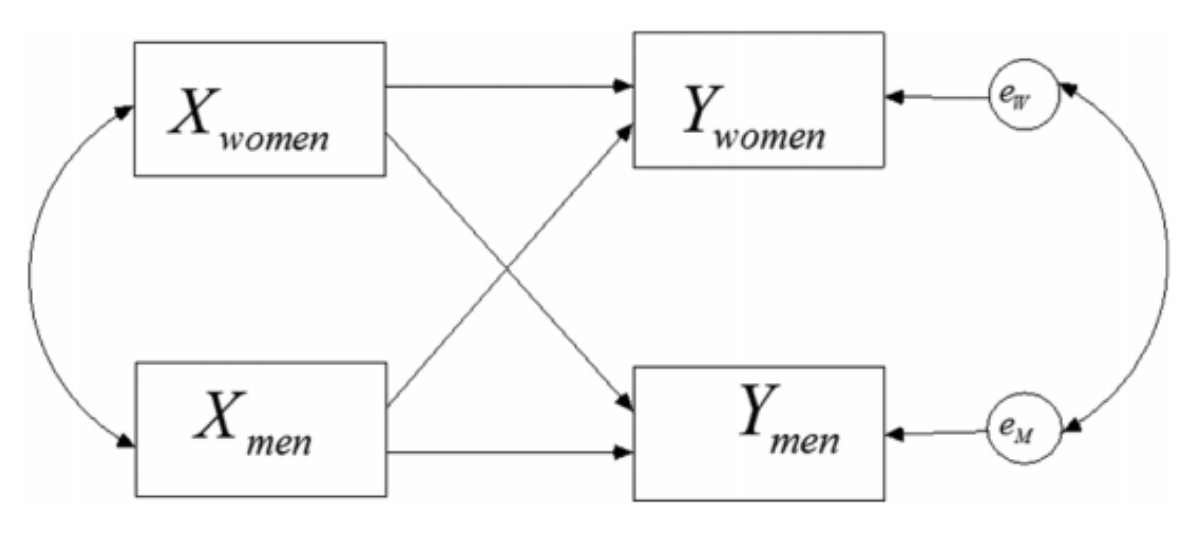
\includegraphics[width=400px]{figures/APIM_figure} \caption{Basic actor-partner interdependence model (APIM) depiction.}\label{fig:apim}
\end{figure}

This study sought to detect whether partners' objectification of one
another affected state self-objectification (SSO). Specifically, we were
interested in testing the relationship between state-other
objectification and SSO, and how SSO in turn, may or may not affect
feelings of inauthenticity during the interaction. In addition, we also
tested if the effect of other-objectification in an interaction on SSO
is only present for those women who are high in trait
self-objectification (moderation effect). Further, we investigated the
relationships between experiencing interaction inauthenticity and
relationship agency, career aspirations, and cognitive performance.

While past studies investigating objectification in interactions used
dyadic path analysis (Garcia et al., 2016), the current study used
multilevel modeling procedures. Dyadic analyses for distinguishable
dyads (e.g., mixed-gender interacting pairs) is more natural using
Structural Equation Modeling (SEM) than it is for indistinguishable
dyads (e.g., same-gender interacting pairs), as we had in the current
study (Garcia, Kenny, \& Ledermann, 2015; Ledermann \& Kenny, 2017). One
reason for this asymmetry is that, due to the arbitrary distinctions
made between \enquote{partner 1} and \enquote{partner 2} in
indistinguishable dyads, many estimates need to be fixed to be equal
(i.e., paths, variances, covariances, endogenous intercepts, and
exogenous means), but these equality constraints should not then be
considered in the degrees of freedom calculations for fit estimations
(Olsen \& Kenny, 2006). Further, Olsen and Kenny (2006) details how a
new independence model and the corresponding fit measure should be
re-calculated for indistinguishable dyads models. The current study used
dyadic multilevel modeling (MLM) to test all relationships, moderation,
and mediation patterns. The online supplementary materials found at
\url{https://github.com/kkyuchukova/object-in-action} contain model
estimates obtained using SEM. See Ledermann and Kenny (2017) for a more
complete discussion of the considerations for using SEM versus MLM for
dyadic analysis.

Testing hypotheses and exploring relationships in the current sample of
indistinguishable dyads involved using the Actor-Partner Independence
Model (APIM) approach for each outcome variable. See
Figure~\ref{fig:apim} for a basic APIM model. The APIM includes effects
due to one's own, as well as one's partner's, predictor variables
(\(X\)'s) on the one's own outcome variable (\(Y\)). The current study
deals with indistinguishable dyads, meaning the designation of who is
the \enquote{actor} and who is the \enquote{partner} is arbitrary. In
total we ran five APIM's---one for each outcome variable---to test the
series of the relationships proposed (i.e., for SSO, inauthenticity,
career aspirations, relationship agency, and cognitive performance).

\subsection{Main Results}\label{main-results}

\begin{figure}
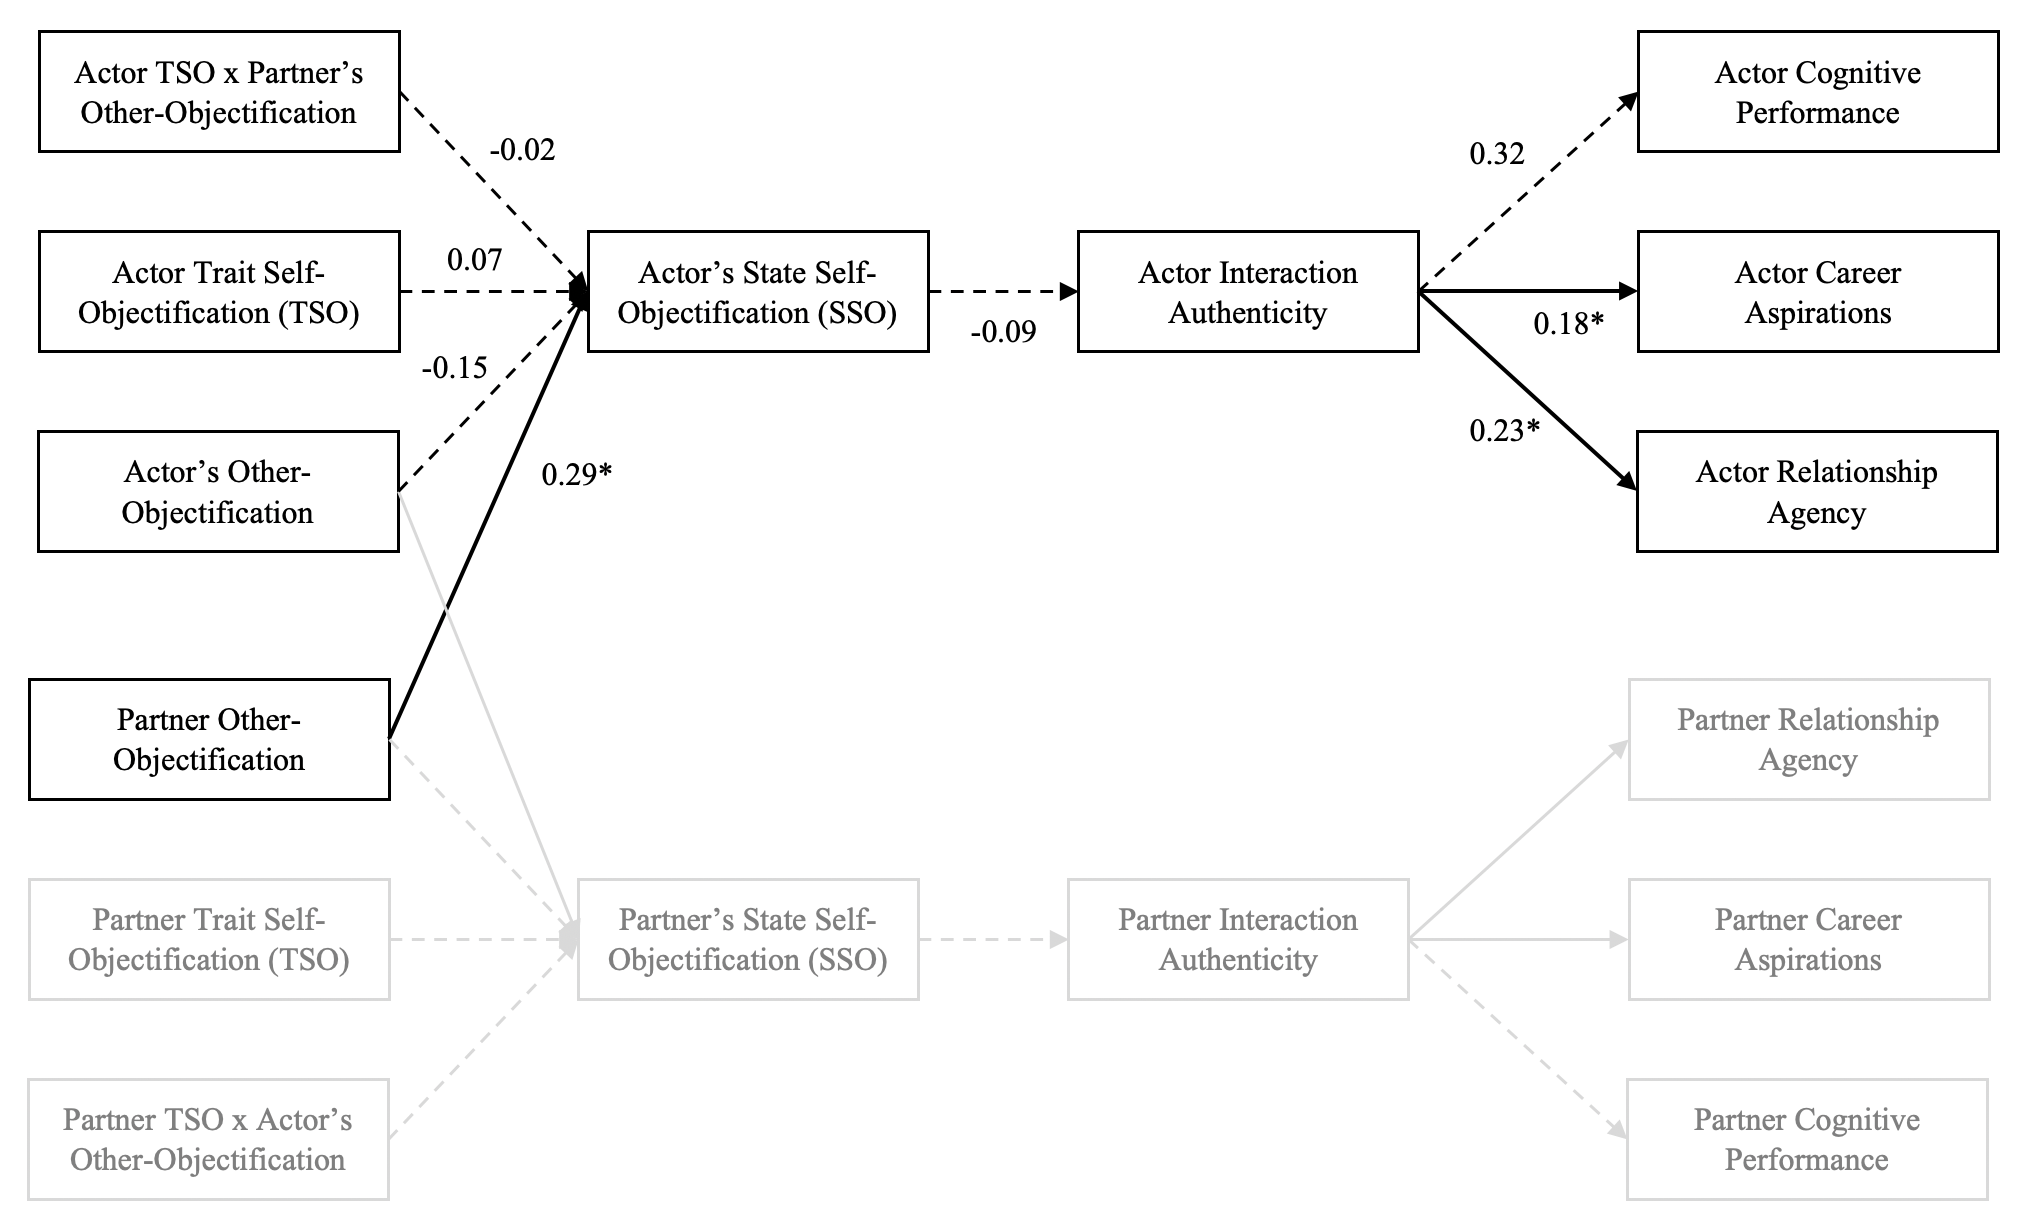
\includegraphics[width=400px]{figures/SEMfigure} \caption{This figure depicts the relationships tested bewteen study variables. The light gray variables represent redundant variables and are shown to emphasize the dyadic nature of the data. The estimates were from obtained from separate MLMs. Sample was controlled for in all models. The effects of TSO, actor other-objectification, and partner other-objectification are from a model where the interaction of TSO and partner other-objectification had been trimmed. *p < .05, dashed lines represent non-significant relationships.}\label{fig:semfigure}
\end{figure}

All relationships between study variables and the MLM estimates are
depicted in Figure~\ref{fig:semfigure}.

First, use used to the APIM to test for evidence of a partner effect of
other objectification and SSO in this sample of same-gender woman-woman
interacting dyads. In Garcia et al. (2016), men's objectification of
women was significantly related to women's SSO, the current study sought
to replicate this partner effect. As expected, the partner effect of
other-objectification on SSO in the current all-women sample was
statistically significant, \emph{b} = 0.29, \emph{SE} = 0.12, \emph{p} =
.019. That is, the extent to which one's partner reported thinking about
a woman's external characteristics more than her internal
characteristics was significantly related to the woman's own reported
feeling more like a body than a full self. Along side the Garcia et al.
(2016) study, there is now evidence that interpersonal objectification
in an actual interpersonal encounter is related to state
self-objectification for women both when the objectifyer is a man and
when the objectifyer is a woman.

In addition to partner other-objectification, this model also included
one's own objectification of their partner (actor
other-objectification), actor trait self-objectification (TSO), and the
interaction of partner other-objectification and TSO. One's own other
objectification had no significant effect on SSO (actor effect of
other-objectification), \emph{b} = -0.16, \emph{SE} = 0.12, \emph{p} =
.210. Further, inconsistent with past findings, there was no
statistically significant interaction of partner's other objectification
and the person's trait self-objectification on SSO, \emph{b} = 0.03,
\emph{SE} = 0.27, \emph{p} = .910. There was also no significant main
effect of trait self-objectification on SSO \emph{b} = 0.07, \emph{SE} =
0.05, \emph{p} = .183. The \(R^2\) of this model (which includes the
partner effect of other-objectification discussed in the previous
paragraph) was only 0.03.

As a test of the potential alternative models discussed in the
introduction---if trait-self-objectification is positively related to
objectifying one's partner---we ran a MLM with other-objectification
predicted by actor TSO. There was no statistically significant
relationship between these two variables, \emph{b} = 0.09, \emph{SE} =
0.06, \emph{p} = .133. We also ran a model with both TSO and SSO
predicting other-objectification, given past theorizing that state
self-objectification might mediate the relationship between TSO and
objectification of fellow women, but there was also no effect of SSO on
other-objectification in this model, \emph{b} = -0.17, \emph{SE} = 0.13,
\emph{p} = .199.

We next moved on to test the link between SSO and interaction
authenticity. There was no significant effect of SSO on interaction
authenticity, although the estimate of this effect was in the
hypothesized negative direction, \emph{b} = -0.09, \emph{SE} = 0.12,
\emph{p} = .431. Because authenticity was a composite score of 9 items,
two of which were interaction specific authenticity items, we also
estimated the pairwise correlations between SSO and all these items
individually. They were all small, ranging from only -0.01 to -0.14.
Although we hypothesized that SSO would mediate the relationship between
partner's other objectification and interaction authenticity, after
finding no relationship between SSO and authenticity, we also tested if
the partner's other objectification had a direct effect on authenticity,
but this effect was not significant, \emph{b} = 0.06, \emph{SE} = 0.12,
\emph{p} = .608 (nor was the total effect of partner's other
objectification on authenticity, \emph{b} = 0.03, \emph{SE} = 0.11,
\emph{p} = .787). Note that these analyses of the relationship between
SSO and inauthenticity in this same-gender sample were considered
exploratory, given that prior research on intragroup interactions points
to mixed possibilities.

Lastly, although there was no evidence that SSO was related to
interaction authenticity in the current sample, we tested if interaction
authenticity (composite of nine items) had effects on cognitive
performance, career aspirations, and relationship agency, as it did in
Garcia et al. (2016). We again used MLM and thus, these effects were
tested in three separate multilevel linear models. There was no
significant effect of interaction authenticity on cognitive performance,
\emph{b} = 0.32, \emph{SE} = 0.28, \emph{p} = .258, but authenticity was
significantly positively related to both career aspirations, \emph{b} =
0.18, \emph{SE} = 0.07, \emph{p} = .010 (\(R^2 =\) 0.04), and
relationship agency, \emph{b} = 0.23, \emph{SE} = 0.12, \emph{p} = .049
(\(R^2 =\) 0.01).

\section{Discussion}\label{discussion}

The current study tested whether the model of interpersonal
objectification and state self-objectification (SSO) used in Garcia et
al. (2016) replicates in a sample of women engaging in actual dyadic
interactions with each other. Although past research has found that
women do objectify other women (Harsey \& Zurbriggen, 2020; Loughnan et
al., 2015; Puvia \& Vaes, 2013), this is the first study to test if
\emph{interpersonal} other-objectification by women during actual
interactions is related to state self-objectification in their
woman-identified interaction partners. As hypothesized, the current
study did find a significant relationship between a woman's interaction
partner's report of having objectified her and her own post-interaction
feelings of self-objectification. That is, there was a significant
partner effect of other-objectification on SSO. This effect extends the
equivalent relationship found in mixed-gender interactions to the
context of same-gender interactions between women. Thus, evidence
suggests that it is not only the real or imagined male gaze that is
related to women's state self-objectification, but there is now also
evidence that being objectified by another woman could be related to
women's SSO, at least in the context of a scenario where they know they
are being evaluated as a potential dating partner.

As is the case in all correlational studies, we cannot be sure about the
causal direction between other-objectification and SSO. The linear model
used by the current study implies that being objectified by a woman
leads women to self-objectify, but it could be that women's SSO causes
them to be objectified by their interaction partner. This latter
interpretation is possible given the empirical evidence that it is
\emph{women's} state self-objectification that relates to being
objectified by one's partner---men partners (Garcia et al., 2016) and
now women partners. Objectification Theory (Fredrickson \& Roberts,
1997), as well as some past experimental studies (for example, Saguy et
al., 2010), suggest that the causal flow is from other-objectification
to SSO. Other studies, especially those investigating explicitly women
objectifying other women (Puvia \& Vaes, 2013), have relatedly found
evidence that women's \emph{trait} self-objectification is related to
women objectifying (dehumanizing) other women and this link is mediated
by \emph{state} self-objectification. The process of interpersonal
objectification among women could also contain a feedback loop. That is,
perhaps we tend to objectify other women who objectify us and through a
process of TSO causing SSO which in turn causes objectification of one's
partner, which in turn causes one's partner to objectify us. However,
the current study does not provide any evidence of the TSO to
other-objectification link---TSO was not significantly correlated with
SSO and, further, actor's other-objectification was not correlated with
partner's other-objectification.

Where the results of the current study diverge most notably from the
results of studies testing interpersonal objectification among
mixed-gender dyads is the lack of evidence for relationships between SSO
and interaction inauthenticity. This is somewhat surprising given the
extant evidence linking SSO and cognitive functioning (B. L. Fredrickson
et al., 1998; and see Moradi \& Huang, 2008 for a review; Quinn,
Chaudoir, \& Kallen, 2011) and the research on interpersonal
other-objectification and cognitive functioning (Garcia et al., 2016;
Gervais et al., 2011; Logel et al., 2009). This lack of evidence could
potentially signal diverging processes between women's experiences with
interpersonal objectification from men and interpersonal objectification
from women. There is quite a bit of evidence suggesting that the male
gaze is particularly detrimental (Calogero, 2004; Fredrickson \&
Roberts, 1997; Gervais et al., 2011), and perhaps the
self-objectification experienced within an interaction with a women is
qualitatively different, and perhaps not as harmful, as the state
self-objectification experienced within an interaction with a man.
However, as a strong note of caution, it is best not to interpret a null
result as evidence of no relationship and more research on interpersonal
objectification among women is needed.

The lack of evidence for a relationship between SSO and interaction
authenticity is surprising and again, should not be interpreted as
evidence of no relationship. It should be noted that the estimate of
this relationship was small (close to zero), but in the negative
direction. If it is the case that there is a smaller (i.e., weaker) or
zero connection between women's feelings of SSO and inauthenticity in
interactions with other women than in interactions with men, models of
interpersonal objectification, like the SIMO (Gervais et al., 2020),
could be extended by including gender of the objectifyer/interaction
partner as a moderator. Inauthenticity could be added as a potential
moderated mediating factor to help understand the circumstances that
require other-objectification and SSO to have negative consequences for
women. Perhaps one important difference is the lack of a power
differential across gendered lines -- the patriarchal culture is
present, but the interaction partners are not a stigmatizer-stigmatized
pair.

Although the current study did not find a connection between SSO and
authenticity, we did find significant positive relationships between
authenticity and relationship agency, and authenticity and career
aspirations. The relationship between authenticity and cognitive
functioning was also estimated as positive, but was not statistically
significant. Again, due to the lack of connection between SSO and
authenticity, we found no evidence of \emph{indirect} relationships
between SSO and these outcome variables. This evidence of a relationship
between authenticity and the relational outcome variables (i.e.,
relationship agency and career aspirations) provides evidence that
corroborates past findings that felt authenticity in interactions is
important for healthy relationship functioning (Garcia et al., 2016;
Terán et al., 2020) and is related to mental health correlates (Tolman
et al., 2006). Just as authenticity has been found to be important in
intergroup interactions (Brunell et al., 2010; Garcia et al., 2016), we
find more evidence here that disruptions in feelings of authenticity can
negatively impact relationships beyond the current partner. Although the
current study did not find a connection between authenticity and SSO,
this seems theoretically to be a natural connection, and future work
must explore when and how SSO leads to inauthenticity in interpersonal
objectification situations.

\subsection{Limitations and Future
Directions}\label{limitations-and-future-directions}

\subsubsection{Sample Characteristics}\label{sample-characteristics}

In addition to being relatively small and combined across two
institutions, another limitation of the current study sample is that the
it was comprised of Western women only. Being that self-objectification
has been found to be most prevalent in Western culture (Loughnan et al.,
2015) research on objectification conducted outside of Western or
Westernized countries has been scarce (Moradi \& Huang, 2008), although
more recent work has examined objectification from a cross-cultural
framework (Loughnan et al., 2015, Wollast et al. (2020)). Since
\enquote{bodies exist within social and cultural contexts, and hence are
also constructed through sociocultural practices and discourses}
(Fredrickson \& Roberts, 1997, p. 174), it is important to consider how
diverse social identities within unique cultural contexts may inform
sexual objectification phenomenon to test the cross-cultural
applicability of theoretical frameworks (Loughnan et al., 2015).

Further, sexualizing experiences and self-objectification are thought to
begin a very young age, and thus, researchers have only recently begun
to examine such experiences among children (e.g., Holland \& Haslam,
2016; Jongenelis, Byrne, \& Pettigrew, 2014). Considering the fact that
the average mean age of the investigated participants of this current
study was 18.85 years, research among younger and older individuals is
needed, especially because the processes of self-objectification may
change over time (Fredrickson \& Roberts, 1997). It may be valuable to
question the extent to which children, adolescents, or emerging adults
of different races or ethnicities are exposed to varied amounts of
sexualizing content. Further, more longitudinal studies investigating
the developmental experience of interpersonal objectification and
self-objectification are needed.

\subsubsection{Interpersonal Sexual Objectification, Gender, and Sexual
Attraction}\label{interpersonal-sexual-objectification-gender-and-sexual-attraction}

The current sample contained a mixture of heterosexual and
non-heterosexual women, but all participants were asked to think about
and evaluate their partner as a potential dating/romantic partner. We
think that heterosexual women are able to do this with other women as
their target---and there is evidence that they might do this readily
(Puvia \& Vaes, 2013; Strelan \& Hargreaves, 2005)---perhaps they may be
even more apt to activate social comparison processes (Festinger, 1954)
than women who are sexually attracted to other women (non-heterosexual
women). Since both men and women are socialized in a culture that
sexually objectifies women, both men and women may come to internalize
this socialization and sexually objectify women. Indeed, recent research
has found that the more women self-objectify, the more they objectify
other women (Loughnan et al., 2015; Puvia \& Vaes, 2013), although not
to the degree exhibited by men; that is, men were found to objectify
women significantly more than women objectify other women (Strelan \&
Hargreaves, 2005). This differential psychological process between women
with differing sexualities might have served to dampen our ability to
detect relationships.

Previous research has found that when compared to heterosexual women,
lesbian women report less concern with physical appearance (Siever,
1994; Strong, Williamson, Netemeyer, \& Geer, 2000), lower body
surveillance (Hill \& Fischer, 2008), and lower self-objectification
(Noffsinger-Frazier, 2004). However none of these studies examined the
relationship between self-objectification and experiences of sexual
objectification. Thus, it is unclear whether lesbian women indeed
experience similar levels of cultural sexual objectification but
internalize them less than heterosexual women do. Consistent with
previous research, Hill and Fischer (2008) determined that lesbians
exhibited less physical appearance concerns compared to heterosexual
women, however there was no evidence found that lesbian women
self-objectify less than heterosexual women and they did not find that
sexual orientation moderates the relationship between sexual
objectification and self-objectification. This evidence sits in contrast
to older theoretical literature that suggests that lesbians internalize
cultural sexual objectification less than do heterosexual women (Brown,
1987; Pitman, 1999; Rothblum, 1994; Siever, 1994).

\section{Conclusion}\label{conclusion}

The results of this study demonstrate the complex and ambivalent nature
of sexual objectification and additionally highlight the psychological
and social consequences of such objectification processes on women's
social relationships and well-being. These results are quite useful for
promoting mental health, the creation and maintenance of early action
programs for girls and young women, and for scholars and practitioners
to work intentionally to provide the tools necessary to circumvent or
mitigate negative effects on self-objectification to combat such
experiences.

\newpage

\section{References}\label{references}

\begingroup
\setlength{\parindent}{-0.5in} \setlength{\leftskip}{0.5in}

\hypertarget{refs}{}
\hypertarget{ref-argyle1969}{}
Argyle, M., \& Williams, M. (1969). Observer or observed? A reversible
perspective in person perception. \emph{Sociometry}, 396--412.

\hypertarget{ref-R-papaja}{}
Aust, F., \& Barth, M. (2018). \emph{papaja: Create APA manuscripts with
R Markdown}. Retrieved from \url{https://github.com/crsh/papaja}

\hypertarget{ref-Bartky}{}
Bartky, S. (1990). \emph{Femininity and domination: Studies in the
phenomenology of oppression}. Routledge, New York.

\hypertarget{ref-brown1987lesbians}{}
Brown, L. S. (1987). Lesbians, weight, and eating: New analyses and
perspectives. \emph{Lesbian Psychologies: Explorations and Challenges},
294--309.

\hypertarget{ref-brunelletal2010}{}
Brunell, A. B., Kernis, M. H., Goldman, B. M., Heppner, W., Davis, P.,
Cascio, E. V., \& Webster, G. D. (2010). Dispositional authenticity and
romantic relationship functioning. \emph{Personality and Individual
Differences}, \emph{48}(8), 900--905.
doi:\href{https://doi.org/10.1016/j.paid.2010.02.018}{10.1016/j.paid.2010.02.018}

\hypertarget{ref-calogero2004test}{}
Calogero, R. M. (2004). A test of objectification theory: The effect of
the male gaze on appearance concerns in college women. \emph{Psychology
of Women Quarterly}, \emph{28}(1), 16--21.

\hypertarget{ref-calogero2011}{}
Calogero, R. M., Tantleff-Dunn, S. E., \& Thompson, J. (2011).
\emph{Self-objectification in women: Causes, consequences, and
counteractions.} American Psychological Association.

\hypertarget{ref-davies2005clearing}{}
Davies, P. G., Spencer, S. J., \& Steele, C. M. (2005). Clearing the
air: Identity safety moderates the effects of stereotype threat on
women's leadership aspirations. \emph{Journal of Personality and Social
Psychology}, \emph{88}(2), 276.

\hypertarget{ref-deaux1987putting}{}
Deaux, K., \& Major, B. (1987). Putting gender into context: An
interactive model of gender-related behavior. \emph{Psychological
Review}, \emph{94}(3), 369.

\hypertarget{ref-dovidio2006nonverbal}{}
Dovidio, J. F., Hebl, M., Richeson, J. A., \& Shelton, J. N. (2006).
Nonverbal communication, race, and intergroup interaction.

\hypertarget{ref-festinger1954theory}{}
Festinger, L. (1954). A theory of social comparison processes.
\emph{Human Relations}, \emph{7}(2), 117--140.

\hypertarget{ref-fredrickson1998swimsuit}{}
Fredrickson, B. L., Roberts, T.-A., Noll, S. M., Quinn, D. M., \&
Twenge, J. M. (1998). That swimsuit becomes you: Sex differences in
self-objectification, restrained eating, and math performance.
\emph{Journal of Personality and Social Psychology}, \emph{75}(1), 269.

\hypertarget{ref-robertsfredrickson}{}
Fredrickson, \& Roberts. (1997). Objectification theory: Toward
understanding women's lived experiences and mental health risks.
\emph{Psychology of Women Quarterly}, \emph{21}(2), 173--206.

\hypertarget{ref-garcia2016objectification}{}
Garcia, R. L., Earnshaw, V. A., \& Quinn, D. M. (2016). Objectification
in action: Self-and other-objectification in mixed-sex interpersonal
interactions. \emph{Psychology of Women Quarterly}, \emph{40}(2),
213--228.

\hypertarget{ref-garcia2015moderation}{}
Garcia, R. L., Kenny, D. A., \& Ledermann, T. (2015). Moderation in the
actor--partner interdependence model. \emph{Personal Relationships},
\emph{22}(1), 8--29.

\hypertarget{ref-gay2010my}{}
Gay, R. K., \& Castano, E. (2010). My body or my mind: The impact of
state and trait objectification on women's cognitive resources.
\emph{European Journal of Social Psychology}, \emph{40}(5), 695--703.

\hypertarget{ref-gervais2013my}{}
Gervais, S. J., Holland, A. M., \& Dodd, M. D. (2013). My eyes are up
here: The nature of the objectifying gaze toward women. \emph{Sex
Roles}, \emph{69}(11-12), 557--570.

\hypertarget{ref-gervais2020social}{}
Gervais, S. J., Sáez, G., Riemer, A. R., \& Klein, O. (2020). The social
interaction model of objectification: A process model of goal-based
objectifying exchanges between men and women. \emph{British Journal of
Social Psychology}, \emph{59}(1), 248--283.

\hypertarget{ref-gervais2011you}{}
Gervais, S. J., Vescio, T. K., \& Allen, J. (2011). When what you see is
what you get: The consequences of the objectifying gaze for women and
men. \emph{Psychology of Women Quarterly}, \emph{35}(1), 5--17.

\hypertarget{ref-grayobrien2007}{}
Gray, M. P., \& OBrien, K. M. (2007). Advancing the assessment of
women's career choices: The career aspiration scale. \emph{Journal of
Career Assessment - J CAREER ASSESSMENT}, \emph{15}, 317--337.
doi:\href{https://doi.org/10.1177/1069072707301211}{10.1177/1069072707301211}

\hypertarget{ref-harsey2020men}{}
Harsey, S. J., \& Zurbriggen, E. L. (2020). Men and women's
self-objectification, objectification of women, and sexist beliefs.
\emph{Self and Identity}, 1--8.

\hypertarget{ref-hebl2005promoting}{}
Hebl, M. R., \& Dovidio, J. F. (2005). Promoting the ``social'' in the
examination of social stigmas. \emph{Personality and Social Psychology
Review}, \emph{9}(2), 156--182.

\hypertarget{ref-henley1977body}{}
Henley, N. (1977). \emph{Body politics: Power, sex, and nonverbal
communication}. Prentice Hall.

\hypertarget{ref-hill2008examining}{}
Hill, M. S., \& Fischer, A. R. (2008). Examining objectification theory:
Lesbian and heterosexual women's experiences with sexual-and
self-objectification. \emph{The Counseling Psychologist}, \emph{36}(5),
745--776.

\hypertarget{ref-holland2016}{}
Holland, E., \& Haslam, N. (2016). Cute little things: The
objectification of prepubescent girls. \emph{Psychology of Women
Quarterly}, \emph{40}(1), 108--119.

\hypertarget{ref-jongenelis2014}{}
Jongenelis, M. I., Byrne, S. M., \& Pettigrew, S. (2014).
Self-objectification, body image disturbance, and eating disorder
symptoms in young australian children. \emph{Body Image}, \emph{11}(3),
290--302.

\hypertarget{ref-kahalon2018don}{}
Kahalon, R., Shnabel, N., \& Becker, J. C. (2018). ``Don't bother your
pretty little head'' appearance compliments lead to improved mood but
impaired cognitive performance. \emph{Psychology of Women Quarterly},
\emph{42}(2), 136--150.

\hypertarget{ref-kenny2006dyadic}{}
Kenny, D. A., Kashy, D. A., \& Cook, W. L. (2006). \emph{Dyadic data
analysis}. Guilford press.

\hypertarget{ref-ledermann2017analyzing}{}
Ledermann, T., \& Kenny, D. A. (2017). Analyzing dyadic data with
multilevel modeling versus structural equation modeling: A tale of two
methods. \emph{Journal of Family Psychology}, \emph{31}(4), 442.

\hypertarget{ref-logel2009interacting}{}
Logel, C., Walton, G. M., Spencer, S. J., Iserman, E. C., Hippel, W.
von, \& Bell, A. E. (2009). Interacting with sexist men triggers social
identity threat among female engineers. \emph{Journal of Personality and
Social Psychology}, \emph{96}(6), 1089.

\hypertarget{ref-loughnan2017internalizing}{}
Loughnan, S., Baldissarri, C., Spaccatini, F., \& Elder, L. (2017).
Internalizing objectification: Objectified individuals see themselves as
less warm, competent, moral, and human. \emph{British Journal of Social
Psychology}, \emph{56}(2), 217--232.

\hypertarget{ref-loughnan2015exploring}{}
Loughnan, S., Fernandez-Campos, S., Vaes, J., Anjum, G., Aziz, M.,
Harada, C., \ldots{} Tsuchiya, K. (2015). Exploring the role of culture
in sexual objectification: A seven nations study. \emph{Revue
Internationale de Psychologie Sociale}, \emph{28}(1), 125--152.

\hypertarget{ref-mcfarlin1984remote}{}
McFarlin, D. B., \& Blascovich, J. (1984). On the remote associates test
(rat) as an alternative to illusory performance feedback: A
methodological note. \emph{Basic and Applied Social Psychology},
\emph{5}(3), 223--229.

\hypertarget{ref-meltzer2020women}{}
Meltzer, A. L. (2020). Women can benefit from sexual and physical
valuation in the context of a romantic relationship. \emph{Personality
and Social Psychology Bulletin}, \emph{46}(2), 243--257.

\hypertarget{ref-moradi2008}{}
Moradi, B., \& Huang, Y.-P. (2008). Objectification theory and
psychology of women: A decade of advances and future directions.
\emph{Psychology of Women Quarterly}, \emph{32}(4), 377--398.

\hypertarget{ref-morry2001magazine}{}
Morry, M. M., \& Staska, S. L. (2001). Magazine exposure:
Internalization, self-objectification, eating attitudes, and body
satisfaction in male and female university students. \emph{Canadian
Journal of Behavioural Science/Revue Canadienne Des Sciences Du
Comportement}, \emph{33}(4), 269.

\hypertarget{ref-nadal2012effects}{}
Nadal, K. L., \& Haynes, K. (2012). Women's psychology. women and mental
disorders. In N. Lundberg-Love P. K. \& M. A. Paludi (Eds.), (pp.
87--101). Praeger/ABC-CLIO.

\hypertarget{ref-noffsinger2004objectification}{}
Noffsinger-Frazier, N. A. (2004). \emph{Objectification theory and
disordered eating: The impact of feminist identification,
internalization of sociocultural standards of appearance, and sexual
orientation} (PhD thesis). The University of Memphis.

\hypertarget{ref-nollfredrickson1998}{}
Noll, S., \& Fredrickson, B. (1998). A mediational model linking
self-objectification, body shame, and disordered eating.
\emph{Psychology of Women Quarterly}, \emph{22}, 623--636.
doi:\href{https://doi.org/10.1111/j.1471-6402.1998.tb00181.x}{10.1111/j.1471-6402.1998.tb00181.x}

\hypertarget{ref-olsen2006structural}{}
Olsen, J. A., \& Kenny, D. A. (2006). Structural equation modeling with
interchangeable dyads. \emph{Psychological Methods}, \emph{11}(2), 127.

\hypertarget{ref-patil2016statistical}{}
Patil, P., Peng, R. D., \& Leek, J. T. (2016). A statistical definition
for reproducibility and replicability. \emph{BioRxiv}, 066803.

\hypertarget{ref-pearson2008fragility}{}
Pearson, A. R., West, T. V., Dovidio, J. F., Powers, S. R., Buck, R., \&
Henning, R. (2008). The fragility of intergroup relations: Divergent
effects of delayed audiovisual feedback in intergroup and intragroup
interaction. \emph{Psychological Science}, \emph{19}(12), 1272--1279.

\hypertarget{ref-R-nlme}{}
Pinheiro, J., Bates, D., DebRoy, S., Sarkar, D., \& R Core Team. (2017).
\emph{nlme: Linear and nonlinear mixed effects models}. Retrieved from
\url{https://CRAN.R-project.org/package=nlme}

\hypertarget{ref-pitman1999body}{}
Pitman, G. E. (1999). Body image, compulsory heterosexuality, and
internalized homophobia. \emph{Journal of Lesbian Studies}, \emph{3}(4),
129--139.

\hypertarget{ref-puvia2013being}{}
Puvia, E., \& Vaes, J. (2013). Being a body: Women's appearance related
self-views and their dehumanization of sexually objectified female
targets. \emph{Sex Roles}, \emph{68}(7-8), 484--495.

\hypertarget{ref-quinnetal}{}
Quinn, D. M., Chaudoir, S. R., \& Kallen, R. W. (2011). Performance and
flow: A review and integration of self-objectification research.
\emph{Self-Objectification in Women: Causes, Consequences, and
Counteractions.}, 119--138.
doi:\href{https://doi.org/10.1037/12304-006}{10.1037/12304-006}

\hypertarget{ref-quinn2011performance}{}
Quinn, D. M., Chaudoir, S. R., \& Kallen, R. W. (2011). Performance and
flow: A review and integration of self-objectification research.

\hypertarget{ref-R-base}{}
R Core Team. (2017). \emph{R: A language and environment for statistical
computing}. Vienna, Austria: R Foundation for Statistical Computing.
Retrieved from \url{https://www.R-project.org/}

\hypertarget{ref-R-psych}{}
Revelle, W. (2017). \emph{Psych: Procedures for psychological,
psychometric, and personality research}. Evanston, Illinois:
Northwestern University. Retrieved from
\url{https://CRAN.R-project.org/package=psych}

\hypertarget{ref-richeson2003prejudice}{}
Richeson, J. A., \& Shelton, J. N. (2003). When prejudice does not pay:
Effects of interracial contact on executive function.
\emph{Psychological Science}, \emph{14}(3), 287--290.

\hypertarget{ref-riemer2020self}{}
Riemer, A. R., Sáez, G., Brock, R., \& Gervais, S. J. (2020).
Self-fulfilling objectification in relationships: The effects of men's
objectifying expectations on women's self-objectification during
conflict in romantic relationships. \emph{Self and Identity}, 1--7.

\hypertarget{ref-rollero2016bringing}{}
Rollero, C. (2016). Bringing objectification into social relationships
research: Is self-objectification harmful for authenticity? \emph{The
Spanish Journal of Psychology}, (19), 1--7.

\hypertarget{ref-rothblum1994lesbians}{}
Rothblum, E. (1994). Lesbians and physical appearance which model
applies? \emph{Lesbian and Gay Psychology: Theory, Research, and
Clinical Applications}, \emph{1}, 84.

\hypertarget{ref-saguyetal2010}{}
Saguy, T., Quinn, D., F Dovidio, J., \& Pratto, F. (2010). Interacting
like a body: Objectification can lead women to narrow their presence in
social interactions. \emph{Psychological Science}, \emph{21}, 178--82.
doi:\href{https://doi.org/10.1177/0956797609357751}{10.1177/0956797609357751}

\hypertarget{ref-sanchez2008romance}{}
Sanchez, D. T., \& Broccoli, T. L. (2008). The romance of
self-objectification: Does priming romantic relationships induce states
of self-objectification among women? \emph{Sex Roles}, \emph{59}(7-8),
545--554.

\hypertarget{ref-shelton2005expecting}{}
Shelton, J. N., Richeson, J. A., \& Salvatore, J. (2005). Expecting to
be the target of prejudice: Implications for interethnic interactions.
\emph{Personality and Social Psychology Bulletin}, \emph{31}(9),
1189--1202.

\hypertarget{ref-siever1994sexual}{}
Siever, M. D. (1994). Sexual orientation and gender as factors in
socioculturally acquired vulnerability to body dissatisfaction and
eating disorders. \emph{Journal of Consulting and Clinical Psychology},
\emph{62}(2), 252.

\hypertarget{ref-R-apaTables}{}
Stanley, D. (2018). \emph{ApaTables: Create american psychological
association (apa) style tables}. Retrieved from
\url{https://CRAN.R-project.org/package=apaTables}

\hypertarget{ref-strelan2005women}{}
Strelan, P., \& Hargreaves, D. (2005). Women who objectify other women:
The vicious circle of objectification? \emph{Sex Roles},
\emph{52}(9-10), 707--712.

\hypertarget{ref-strelan2018birds}{}
Strelan, P., \& Pagoudis, S. (2018). Birds of a feather flock together:
The interpersonal process of objectification within intimate
heterosexual relationships. \emph{Sex Roles}, \emph{79}(1-2), 72--82.

\hypertarget{ref-strong2000eating}{}
Strong, S. M., Williamson, D. A., Netemeyer, R. G., \& Geer, J. H.
(2000). Eating disorder symptoms and concerns about body differ as a
function of gender and sexual orientation. \emph{Journal of Social and
Clinical Psychology}, \emph{19}(2), 240--255.

\hypertarget{ref-teran2020relational}{}
Terán, L., Jiao, J., \& Aubrey, J. S. (2020). The relational burden of
objectification: Exploring how past experiences of interpersonal sexual
objectification are related to relationship competencies. \emph{Sex
Roles}, 1--16.

\hypertarget{ref-tolman2006looking}{}
Tolman, D. L., Impett, E. A., Tracy, A. J., \& Michael, A. (2006).
Looking good, sounding good: Femininity ideology and adolescent girls'
mental health. \emph{Psychology of Women Quarterly}, \emph{30}(1),
85--95.

\hypertarget{ref-R-tidyverse}{}
Wickham, H. (2017). \emph{Tidyverse: Easily install and load the
'tidyverse'}. Retrieved from
\url{https://CRAN.R-project.org/package=tidyverse}

\hypertarget{ref-wollast2020cultural}{}
Wollast, R., Riemer, A. R., Gervais, S. J., Grigoryan, L., Bernard, P.,
\& Klein, O. (2020). How cultural orientation and self-compassion shape
objectified body consciousness for women from america, belgium, russia,
and thailand. \emph{Self and Identity}, 1--21.

\hypertarget{ref-R-knitr}{}
Xie, Y. (2015). \emph{Dynamic documents with R and knitr} (2nd ed.).
Boca Raton, Florida: Chapman; Hall/CRC. Retrieved from
\url{https://yihui.name/knitr/}

\hypertarget{ref-R-rmarkdown}{}
Xie, Y., Allaire, J., \& Grolemund, G. (2018). \emph{R markdown: The
definitive guide}. Boca Raton, Florida: Chapman; Hall/CRC. Retrieved
from \url{https://bookdown.org/yihui/rmarkdown}

\hypertarget{ref-yilmaz2019whose}{}
Yilmaz, T., \& Bozo, Ö. (2019). Whose gaze is more objectifying? An
experimental study of college women's state self-objectification, body
shame, negative mood, and body dissatisfaction. \emph{Mediterranean
Journal of Clinical Psychology}, \emph{7}(2).

\hypertarget{ref-zurbriggen2011self}{}
Zurbriggen, E. L., Ramsey, L. R., \& Jaworski, B. K. (2011). Self-and
partner-objectification in romantic relationships: Associations with
media consumption and relationship satisfaction. \emph{Sex Roles},
\emph{64}(7-8), 449--462.

\endgroup


\end{document}
